\chapter{Block Architecture}

\section{Functional Specification}

The pulse channel module generates precisely timed laser pulses using user-defined configurations, base waveforms, and a fixed sequence length. It relies on Xilinx block RAM IPs, a robust state machine, and versatile interfaces to produce a 16-bit waveform for an external 16-bit DAC.

Each pulse has symmetrical rise and fall edges, so the design only stores the rising edge data in one memory block. This decision reduces memory usage and simplifies the waveform generation process by eliminating redundant information. Another RAM block holds the complete waveform definition, including critical details such as start times. This separation allows for dynamic updates to the base shape without altering existing data. The benefit of this approach is that it minimizes resource usage and makes real-time adjustments easier.

The pulse generator is activated by an external trigger, ensuring that the system is both flexible and responsive. Once triggered, the module reads the RAM-stored configuration, processes the waveform through the state machine, and outputs the corresponding pulse. Multiple waveform variations can be defined, allowing the system to seamlessly transition from one pulse definition to the next until the entire sequence is completed. The resulting 16-bit waveform is then transmitted through the FPGA's AXI-stream interface to the external DAC. Standard signaling protocols such as valid, ready, and last manage data transfer and synchronization, ensuring that the pulse shape is preserved with minimal latency.

All waveform data and parameters are loaded into RAM via a 32-bit data, 12-bit address interface. This interface supports both configuration and monitoring, enabling the module to select between the RAM blocks or perform real-time diagnostics and debugging. This flexibility allows for rapid reconfiguration and continuous system oversight, which is essential for maintaining its high performance.

Error handling is integrated into the module. Dedicated error signals are generated during pulse generation to detect anomalies and trigger immediate responses. Pipeline delays are carefully managed to ensure signal synchronization and maintain timing margins across the data path.

\begin{figure}[h]
    \centering
    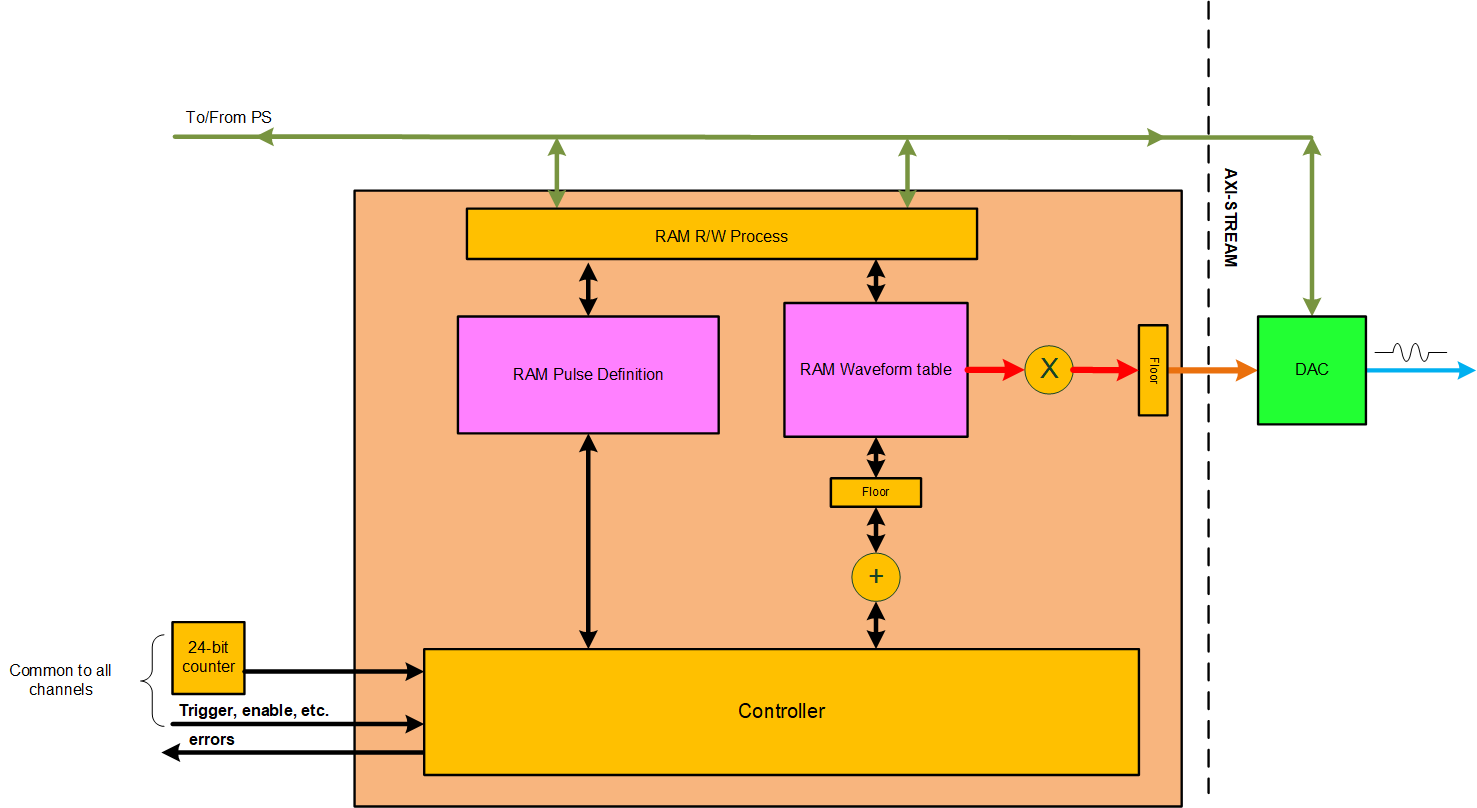
\includegraphics[width=1.0\linewidth]{figures/3.1.png}
    \caption{Block diagram of the pulse channel with two RAMs integrated.}
    \label{fig:block_diagram}
\end{figure}

\section{Setup}

The pulse channel module uses two dual-port memories with Xilinx Block Memory Generator \cite{blockmemgen}, as shown in \autoref{fig:block_diagram}. This design choice allows for dynamic waveform generation with configurable parameters, ensuring system responsiveness through parallel access. One port of each memory is read-only, dedicated to the internal controller for waveform generation. The other port is read-write, enabling data to be loaded and stored efficiently. This setup optimizes memory usage and enhances the module's flexibility and performance.

\subsection{Memory Organization and structure}

The module uses two block memories, each serving a unique purpose for high-speed waveform generation. The pulse definition (PD) memory is a 1024x32-bit dual-port block RAM that stores comprehensive waveform parameters. This allows for reconfiguring waveforms in multiple forms without needing to change data in the hardware. The waveform data is stored in the dual-port 4096x16-bit waveform table (WT) memory. This memory holds the base form of the rising edge of the waveform.

The dual-port configuration of both memories is a critical architectural decision, enabling concurrent access from both external interfaces and internal controls for waveform generation. This parallelism ensures that ongoing pulse generation operations remain unaffected by system configuration updates.

\subsection{Pulse Definition}

\begin{figure}[htbp]
    \centering
    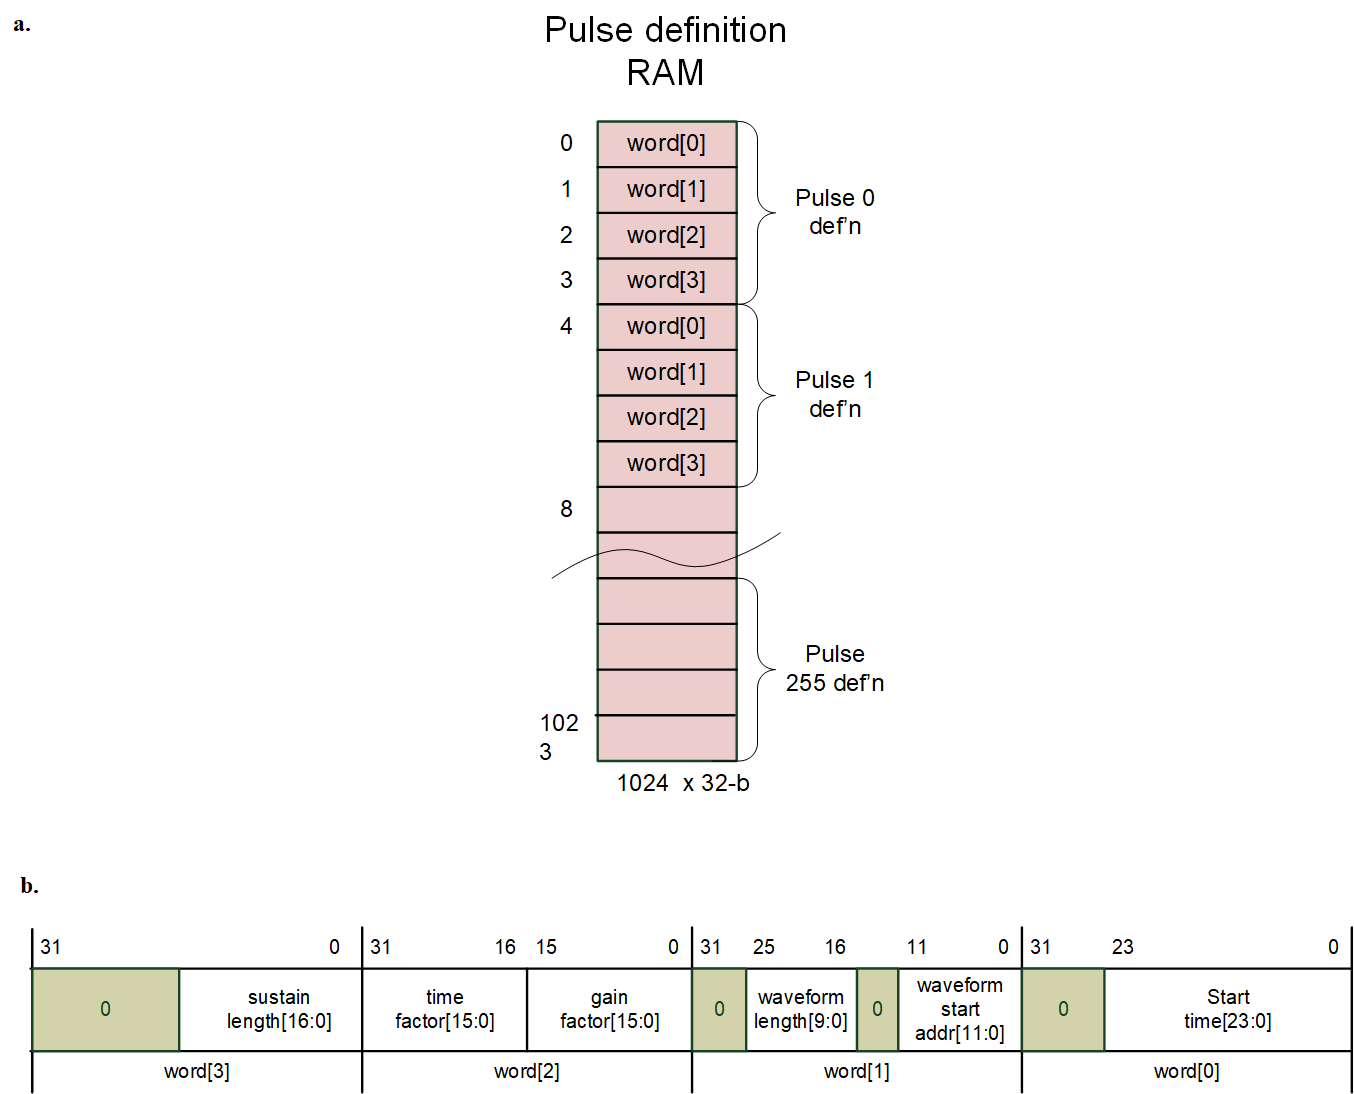
\includegraphics[width=1\linewidth]{figures/3.2.png}
    \caption{\centering{Pulse Definition RAM overall allocation. \textbf{a}, the overall allocation in the memory. \textbf{b}, specific bit-wise allocations of each pulse’s parameter.}}
    \label{fig:pd}
\end{figure}

The pulse definition memory employs a well-organized addressing scheme, where each set of pulse parameters is allocated four consecutive 32-bit memory locations. This means that the parameters for each pulse are stored sequentially, as illustrated in \autoref{fig:pd}a. In other words, each pulse parameter set is 128 bits in length, occupying four consecutive byte addresses. Consequently, the 1024-address memory can accommodate up to 256 pulses per channel, allowing for either unique pulses or variations based on another. This structured approach ensures efficient storage and retrieval of pulse parameters. By organizing the memory in this manner, the system can handle a significant number of pulses while maintaining clarity and ease of access. Each pulse's parameter is defined by \autoref{fig:pd}b and \autoref{tab:pd_param}.

\begin{table}[htbp]
    \centering
    \begin{tabularx}{\textwidth}{|c|X|X|}
        \hline
        Word \# & Name & Description \\
        \hline
        0 & Start Time & Time a pulse should start \\
        \hline
        1 & Waveform Start Address & Starting address of the waveform table memory \\
        \hline
        1 & Gain Factor & Scale the amplitude of the output signal. Within (0,1] \\
        \hline
        2 & Time Factor & Step Size adjusts the rate at which the pulse's rise or fall is executed. In the range [1, waveform length) \\
        \hline
        2 & Waveform Length & Duration of the rise (when the time factor is one). \\
        \hline
        3 & Sustain Length & Duration in 10ns scale of last wave value after rise stage should stay before start the fall stage \\
        \hline
    \end{tabularx}
    \caption{Detailed pulse's parameter set}
    \label{tab:pd_param}
\end{table}



\subsection{Waveform Table}
The waveform table memory is designed to store the base values for the rise of each pulse. As shown in \autoref{fig:wavetable}, each entry in the table consists of a pair of 16-bit values. This design is necessary because at least two values are required to construct the rise or fall of a pulse. A pulse's rise can store up to 2048 32-bit value pairs, or 4096 16-bit data points, in the waveform table memory. The number of value pairs used for each pulse depends on its waveform length. If the waveform length is even, it takes half of the waveform length in value pairs. If the length is odd, it takes the floor of the waveform length divided by 2, plus the lower value of the next pair.
\begin{figure}[htbp]
    \centering
    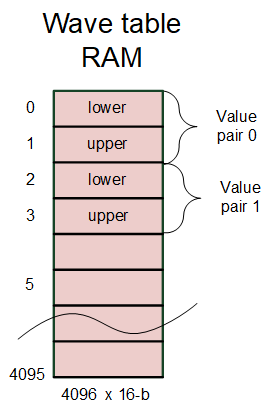
\includegraphics[width=0.30\linewidth]{figures/3.3.png}
    \caption{Memory layout for waveform table}
    \label{fig:wavetable}
\end{figure}
The memory allocation in the waveform table is dynamic, relying on waveform lengths and start addresses from the pulse definition. This design is purpose-built to maximize memory utilization. By adapting the allocated space based on each pulse's requirements, the system can store a single pulse with a maximum length of 4096 data points, or distribute storage among up to 256 pulses where each pulse uses no more than 16 data points on average. This approach ensures that longer pulses receive the space they need while shorter pulses occupy only what is necessary, thus avoiding wasted memory and maintaining efficient resource use.

Furthermore, the waveform table allows multiple pulse definition points to reference the same memory region, given that their start addresses and waveform lengths are identical. This capability is especially beneficial when different scale factors are applied to the same pulse structure. By sharing the memory region, the design avoids redundant storage of waveform data and minimizes additional space usage. 

\section{Procedure}
The module creates precise pulse-shaped waveforms by progressing through a series of well-defined states, shown in \autoref{fig:fsm}. It activates when an external trigger is received from the system while the module is enabled, shown in the bottom left of \autoref{fig:block_diagram}. Upon receiving the trigger, the module loads the necessary data from the pulse definition memory into a set of registers. It then enters a waiting stage and holds until a 24-bit timer reaches the predetermined start time. This approach guarantees that each pulse is generated precisely when needed—a key requirement for synchronization in FPGA applications.
\begin{figure}[htbp]
    \centering
    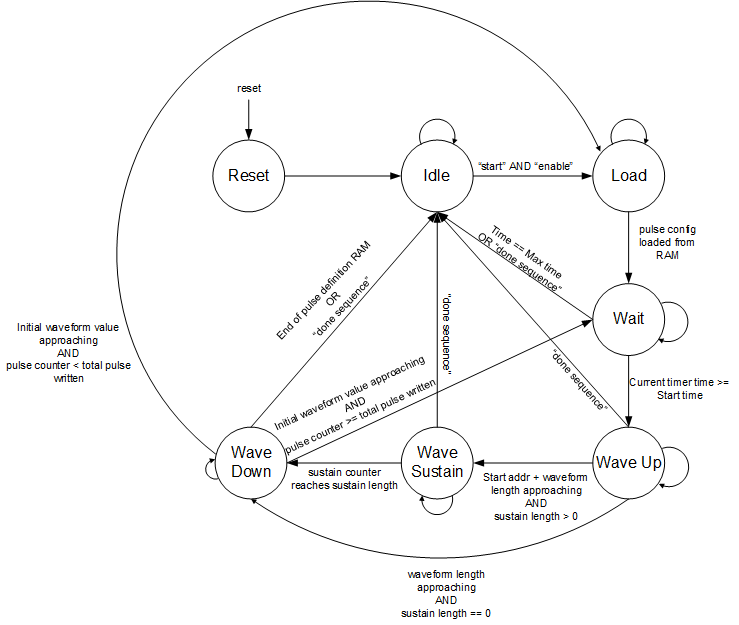
\includegraphics[width=1\linewidth]{figures/3.4.png}
    \caption{State Diagram of the Pulse Channel Module}
    \label{fig:fsm}
\end{figure}
When the timer reaches the start time, the module moves sequentially through the rise, sustain, and fall stages. During these stages, it carefully shapes the pulse by controlling both the waveform table address and its data output using the time and gain factor values. After the fall stage, the module evaluates whether additional pulses remain in the pulse definition memory. If there are more pulses, it immediately loads the next one. Otherwise, it waits for a "done sequence" signal before going idle.

An internal pulse counter monitors the current entry in the pulse definition memory and increments each time a new pulse is loaded. Because each pulse definition spans four memory addresses, the counter increases by four with every update. Another counter tracks the number of clock cycles that the sustain phase has lasted following the rise stage. When this counter reaches the defined sustain length, the state machine transitions to the fall stage. This organized, stage-based design simplifies the control logic while enhancing timing precision and signal integrity. 

In parallel, a separate process manages memory read and write operations via the CPU interface, indicated by the green arrows in \autoref{fig:block_diagram}. The pulse channel module extracts the lower 12 bits from the system address for either pulse definition memory or the waveform table memory. The 12th bit acts as a selection signal, effectively multiplexing data and addresses between these two memories. For the waveform table, each operation transfers a 32-bit value pair, which together constitute one entry. This arrangement yields a total of 2048 available entries for CPU accesses. In contrast, each pulse definition entry spans four 32-bit words. Therefore, it takes four consecutive CPU operations to complete one pulse definition entry. This clear division of memory operations not only ensures efficient and reliable data transfer but also simplifies the addressing scheme, maintaining data integrity and responsiveness in real-time FPGA applications.

\section{Error Handling}

The pulse channel is engineered to be highly robust and resilient, capable of handling both typical user inputs and unusual or invalid parameters. It accounts for common values as well as edge cases that might otherwise disrupt system operation. While the software interface manages most user-induced errors, the built-in error registers and handling mechanisms serve as the final safeguard. This layered approach prevents hazardous inputs from causing system failures, ensuring that the design remains safe and reliable even under unexpected conditions.

To ensure robust performance, several potential cases must be carefully considered. The design guarantees that pulses begin only when the current time meets or exceeds their scheduled start. Special attention is given to the sustain length. For instance, if a pulse definition specifies a flat-top length of zero, the system immediately transitions to the fall stage. The module also keeps track of the total number of generated pulses using the internal pulse counter, which helps maintain proper sequence control. Moreover, if the start time of a subsequent pulse is earlier than that of the previous one, the pulse is omitted to preserve timing integrity.

Additionally, the design manages cases where the waveform start address and length exceed the 4096-entry capacity of the waveform table memory. In such instances, the system either wraps the addresses correctly back into the valid range or triggers an error flag in an 8-bit register, with each bit defined in \autoref{table:erro_regs}. One-hot encoding ensures that the error register uniquely represents each error condition with a single active flag. When a specific error occurs, the system sets only the corresponding flag. This clear mapping simplifies fault diagnosis and reduces ambiguity during troubleshooting. When an error is detected, the system stops waveform generation to prevent the further propagation of invalid data, thereby maintaining overall system integrity. Furthermore, the registers are designed to log and maintain these error events, aiding in prompt debugging and corrective measures. The error registers can be cleared with an external clear flag or by resetting the system. Some registers have no error details assigned yet, allowing for future expandability based on further testing results.
\begin{table}[h]
\setlength{\abovecaptionskip}{5pt}    % Reduces space above caption
\setlength{\belowcaptionskip}{5pt}    % Reduces space below caption
\centering
\caption{Error Registers}
\label{table:erro_regs}
\begin{tabular}{|c|l|}
\hline
Register Bit & Error Details \\
\hline
0 & Wave table RAM overflow \\
\hline
1 & Rise length size $\leq$ 1 (need to min. 2) \\
\hline
2 & Time step bigger than the size of the rise \\
\hline
3 & Amplitude scale $>$ 1 \\
\hline
4 & Time step $<$ 1 \\
\hline
5 & \textit{Not yet assigned} \\
\hline
6 & \textit{Not yet assigned} \\
\hline
7 & \textit{Not yet assigned} \\
\hline
\end{tabular}
\end{table}